\documentclass[11pt]{article}
\usepackage{graphicx, amsmath, amssymb, bm, url, mathtools, natbib, amsthm, setspace}

\pagestyle{plain}
%----------------Page dimensions ----------------
\oddsidemargin 0.0in
\evensidemargin 0.0in
\topmargin -0.75in
\leftmargin 0in
\headheight 0.0in
\headsep 0.5in
%\footheight 0.0in
\footskip 0.5in
\footnotesep 0.0in
\textwidth 6.7in
\textheight 9.5in
%-----------Define Pictures---------------------
\def\picture #1 by #2 (#3){
 \vbox to #2{
   \hrule width #1 height 0pt depth 0pt
   \vfill
   \special{picture #3} % this is the low-level interface
   }
 }
\def\scaledpicture #1 by #2 (#3 scaled #4){{
 \dimen0=#1 \dimen1=#2
 \divide\dimen0 by 1000 \multiply\dimen0 by #4
 \divide\dimen1 by 1000 \multiply\dimen1 by #4
 \picture \dimen0 by \dimen1 (#3 scaled #4)}
 }

\newcommand{\xbar}{\bar{\bm x}}
\newcommand{\tr}{\text{tr}}
\DeclareMathOperator*{\argmin}{arg\,min}
\DeclareMathOperator*{\argmax}{arg\,max}

\title{Numerical Instability of the RDA Classifier}

\author{John A. Ramey and Dean M. Young}

\begin{document}

\newtheorem*{thm}{Theorem}
\newtheorem*{cor}{Corollary}

\bibpunct{(}{)}{;}{a}{,}{,}

\doublespacing

\maketitle

\textbf{The derivation below was initially in my paper entitled ``Another Look at Regularized Discriminant Analysis.'' The reasoning below is flawed though. In my proof, I assume implicitly that the eigenvalues of $\bm A$ are constant as $p$ is incremented. This is not true though: As $p$ increases, the trace of $\bm A$ must increase, so the sum of the eigenvalues of $\bm A$ must also increase. Because the first $q$ eigenvalues of $\bm A$ are positive, while the remainder of them are 0, it must be that the eigenvalues change as $p$ increases. It may be that the reasoning below is solid in many cases, or perhaps in all cases if the constant $c$ is selected correctly in the proof of the theorem below. No matter, in its current form, the proof is flawed.}

\textbf{Holy Grail Question: Assuming $\bm \Gamma$ is a diagonal matrix as defined below, what are the necessary and sufficient conditions for $|\bm A + \bm \Gamma| \rightarrow 0$ so that $\bm A + \bm \Gamma$ is nearly singular as the number of variables included in the model is increased for a fixed rank (sample size)?}

The usual focus of regularization methods employed to stabilize the inverse covariance matrix is often effective in producing well-performing classifiers when $p >> N$. As we have discussed, the shrinkage factor employed in \eqref{eq:sig-rda} involves the average of the eigenvalues of \eqref{eq:sig-lambda}. In this section, we demonstrate that the \emph{RDA} classifier becomes numerically incalculable as $p$ increases for a fixed sample size. First, we present a general result  that if a positive semidefinite matrix $\bm A$ is shrunken towards a diagonal matrix $\bm \Gamma$ consisting of positive diagonal elements less than 1, the shrunken matrix $\bm A + \bm \Gamma$ is nearly positive semidefinite because its determinant goes to 0 as $p \rightarrow \infty$. Next, we demonstrate briefly that the average of the eigenvalues goes to 0 as $p \rightarrow \infty$ for a fixed sample size. The result is that the covariance-matrix shrinkage employed in the \emph{RDA} classifier is ineffective at producing a positive definite covariance matrix estimator, resulting in a numerically incalculable classifier.

\begin{thm}
Let $\bm \Gamma = \text{diag}(\gamma_1, \gamma_2, \ldots, \gamma_p)$ such that $0 < \gamma_j < 1$ for $j = 1, 2, \ldots, p$, and let $\bm A \in \mathbb{R}_{p \times p}^{\ge}$ be symmetric such that $\text{rank}(\bm A) = q < p$ and with eigenvalues $e_1 \ge e_2 \ge \ldots \ge e_p \ge 0$. Then, with $q$ fixed,
\begin{align*}
	\lim_{p \rightarrow \infty} |\bm A + \bm \Gamma| = 0.
\end{align*}
\end{thm}
\begin{proof}
Let $\gamma = \max_j \gamma_j$, and let $c \in \mathbb{R}$ such that $e_1 \le (c - 1) \gamma$. Then, we have that 
	\begin{align*}
		|\bm A + \bm \Gamma| &= \prod_{j = 1}^p (e_j + \gamma_j)\\
%		&\le \prod_{j = 1}^p (e_j + \gamma)\\
		&\le \gamma^{p-q} \prod_{j=1}^q (e_j + \gamma)\\
		&\le c^q\gamma^p.
	\end{align*}
Therefore, as $p \rightarrow \infty$, $|\bm A + \bm \Gamma| \rightarrow 0$ because $c^q\gamma^p \rightarrow 0$.


\end{proof}

\begin{cor}
	 Let $\bm A$ be defined as in the above theorem, and let $\gamma \in (0,1)$. Then, with $q$ fixed,
\begin{align}
	\lim_{p \rightarrow \infty} |\bm A + \gamma \bm I_p| = 0.\label{eq:corollary}
\end{align}
\end{cor}
\begin{proof}
The proof follows directly from the above theorem.
\end{proof}

From \eqref{eq:corollary}, we see that shrinking a large singular covariance matrix $\bm A$ can have no regularization effect on $|\bm A|$.  Supervised classifiers that are functions of the determinant of the covariance matrix, $\widehat{\bm \Sigma}$, can yield invalid results when $p >> N$ because $\text{rank}(\widehat{\bm \Sigma}) \le N - 1$. Now, consider again the RDA classifier in \eqref{eq:rda}. We can see that $D(\bm x) \rightarrow \infty$ as $p \rightarrow \infty$ because $\widehat{\bm\Sigma}_k \rightarrow 0$, $k = 1, \ldots, K$. The natural logarithm is a nuisance function with this classifier. 

As we have shown above, $\lim_{p \rightarrow \infty} \gamma = 0$. Hence, assuming the rank of $\widehat{\bm\Sigma}_k = q_k$, the last $p-q_k$ eigenvalues are 0. This implies that the RDA classifier is not applicable for high-dimensional data.

\section{Example}

To demonstrate the corollary, we first construct a $\bm A \in \mathbb{R}_{p \times p}^{\ge}$, having its first $q = 25$ eigenvalues equal to 1 and the remaining $p - q$ eigenvalues equal to 0. In Figure \ref{fig:log-det}, we see that $\ln |\bm\Sigma + \gamma \bm I_p|$ approaches $-\infty$ quickly for small values of $\gamma$ but is still finite for larger values of $\gamma$. In Figure 2, we see further supportive evidence of our main result for larger values of $\gamma$. For example, $\ln |\bm\Sigma + \gamma \bm I_p|$ is numerically $-\infty$ for $p \ge 400$ with $\gamma = 0.1$.

\begin{figure}[htbp]
\begin{center}
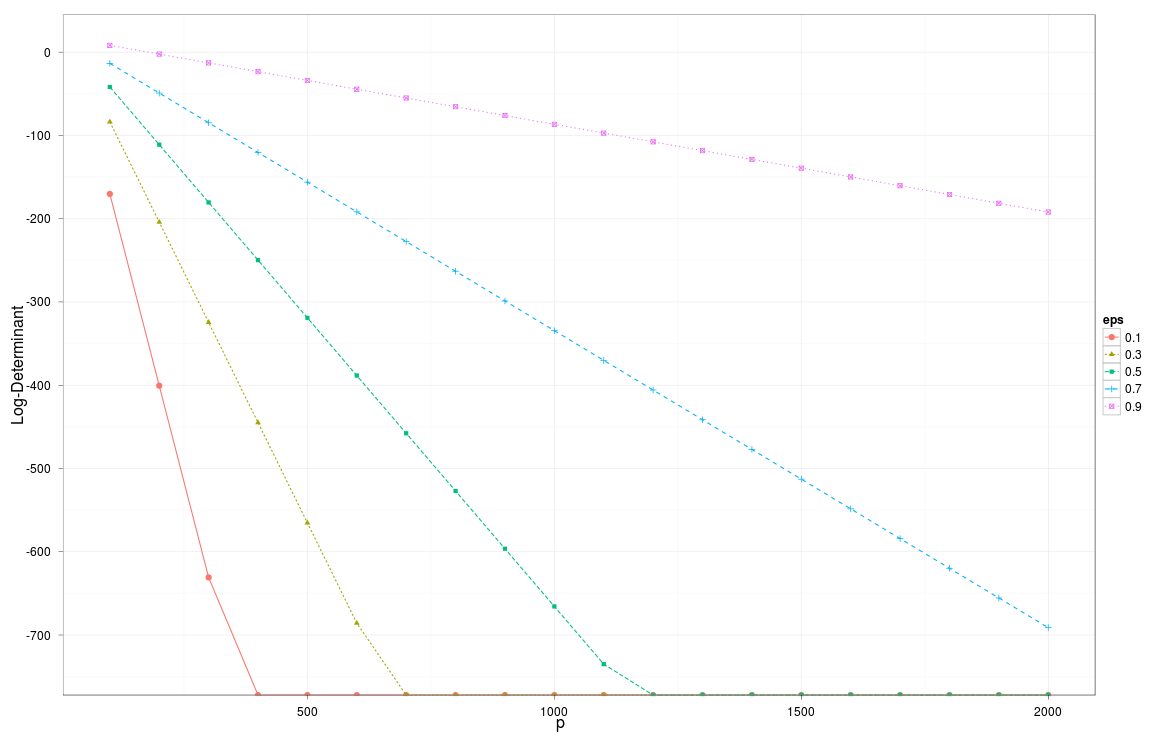
\includegraphics[scale = 0.45]{log-determinant}
\caption{For various values of $\gamma$, we plot $\ln |\bm\Sigma + \gamma \bm I_p|$ as a function of $p$ with rank$(\bm\Sigma)$ fixed at 25. The points on the lower edge of the graph are numerically $-\infty$.}
\label{fig:log-det}
\end{center}
\end{figure}

% The following graphics are produced with the R code:
%library('plyr')
%library('ggplot2')
%
%eps <- c(0.1, 0.3, 0.5, 0.7, 0.9)
%p <- seq.int(100, 2000, by = 100)
%grid <- expand.grid(eps = eps, p = p)
%
%r <- 25
%results_25 <- ddply(grid, .(eps, p), function(g) {
%  log(det(diag(g$eps + c(rep(1, r), rep(0, g$p - r)))))
%})
%names(results_25) <- c("eps", "p", "det")
%results_25$eps <- factor(results_25$eps)
%gp <- ggplot(results_25, aes(x = p, y = det, group = eps, color = eps, linetype = eps))
%gp <- gp + geom_line(size = 2) + geom_point(aes(shape = eps), size = 2)
%gp <- gp + ylab("Log-Determinant")
%gp + theme_set(theme_bw())
%


\end{document}